\newpage
\section{Class diagram}
\label{sec:class_diagram}

\fxnote{Meget af det følgende burde genereres af doxygen - JH}
\begin{figure}[H]
	\centering
	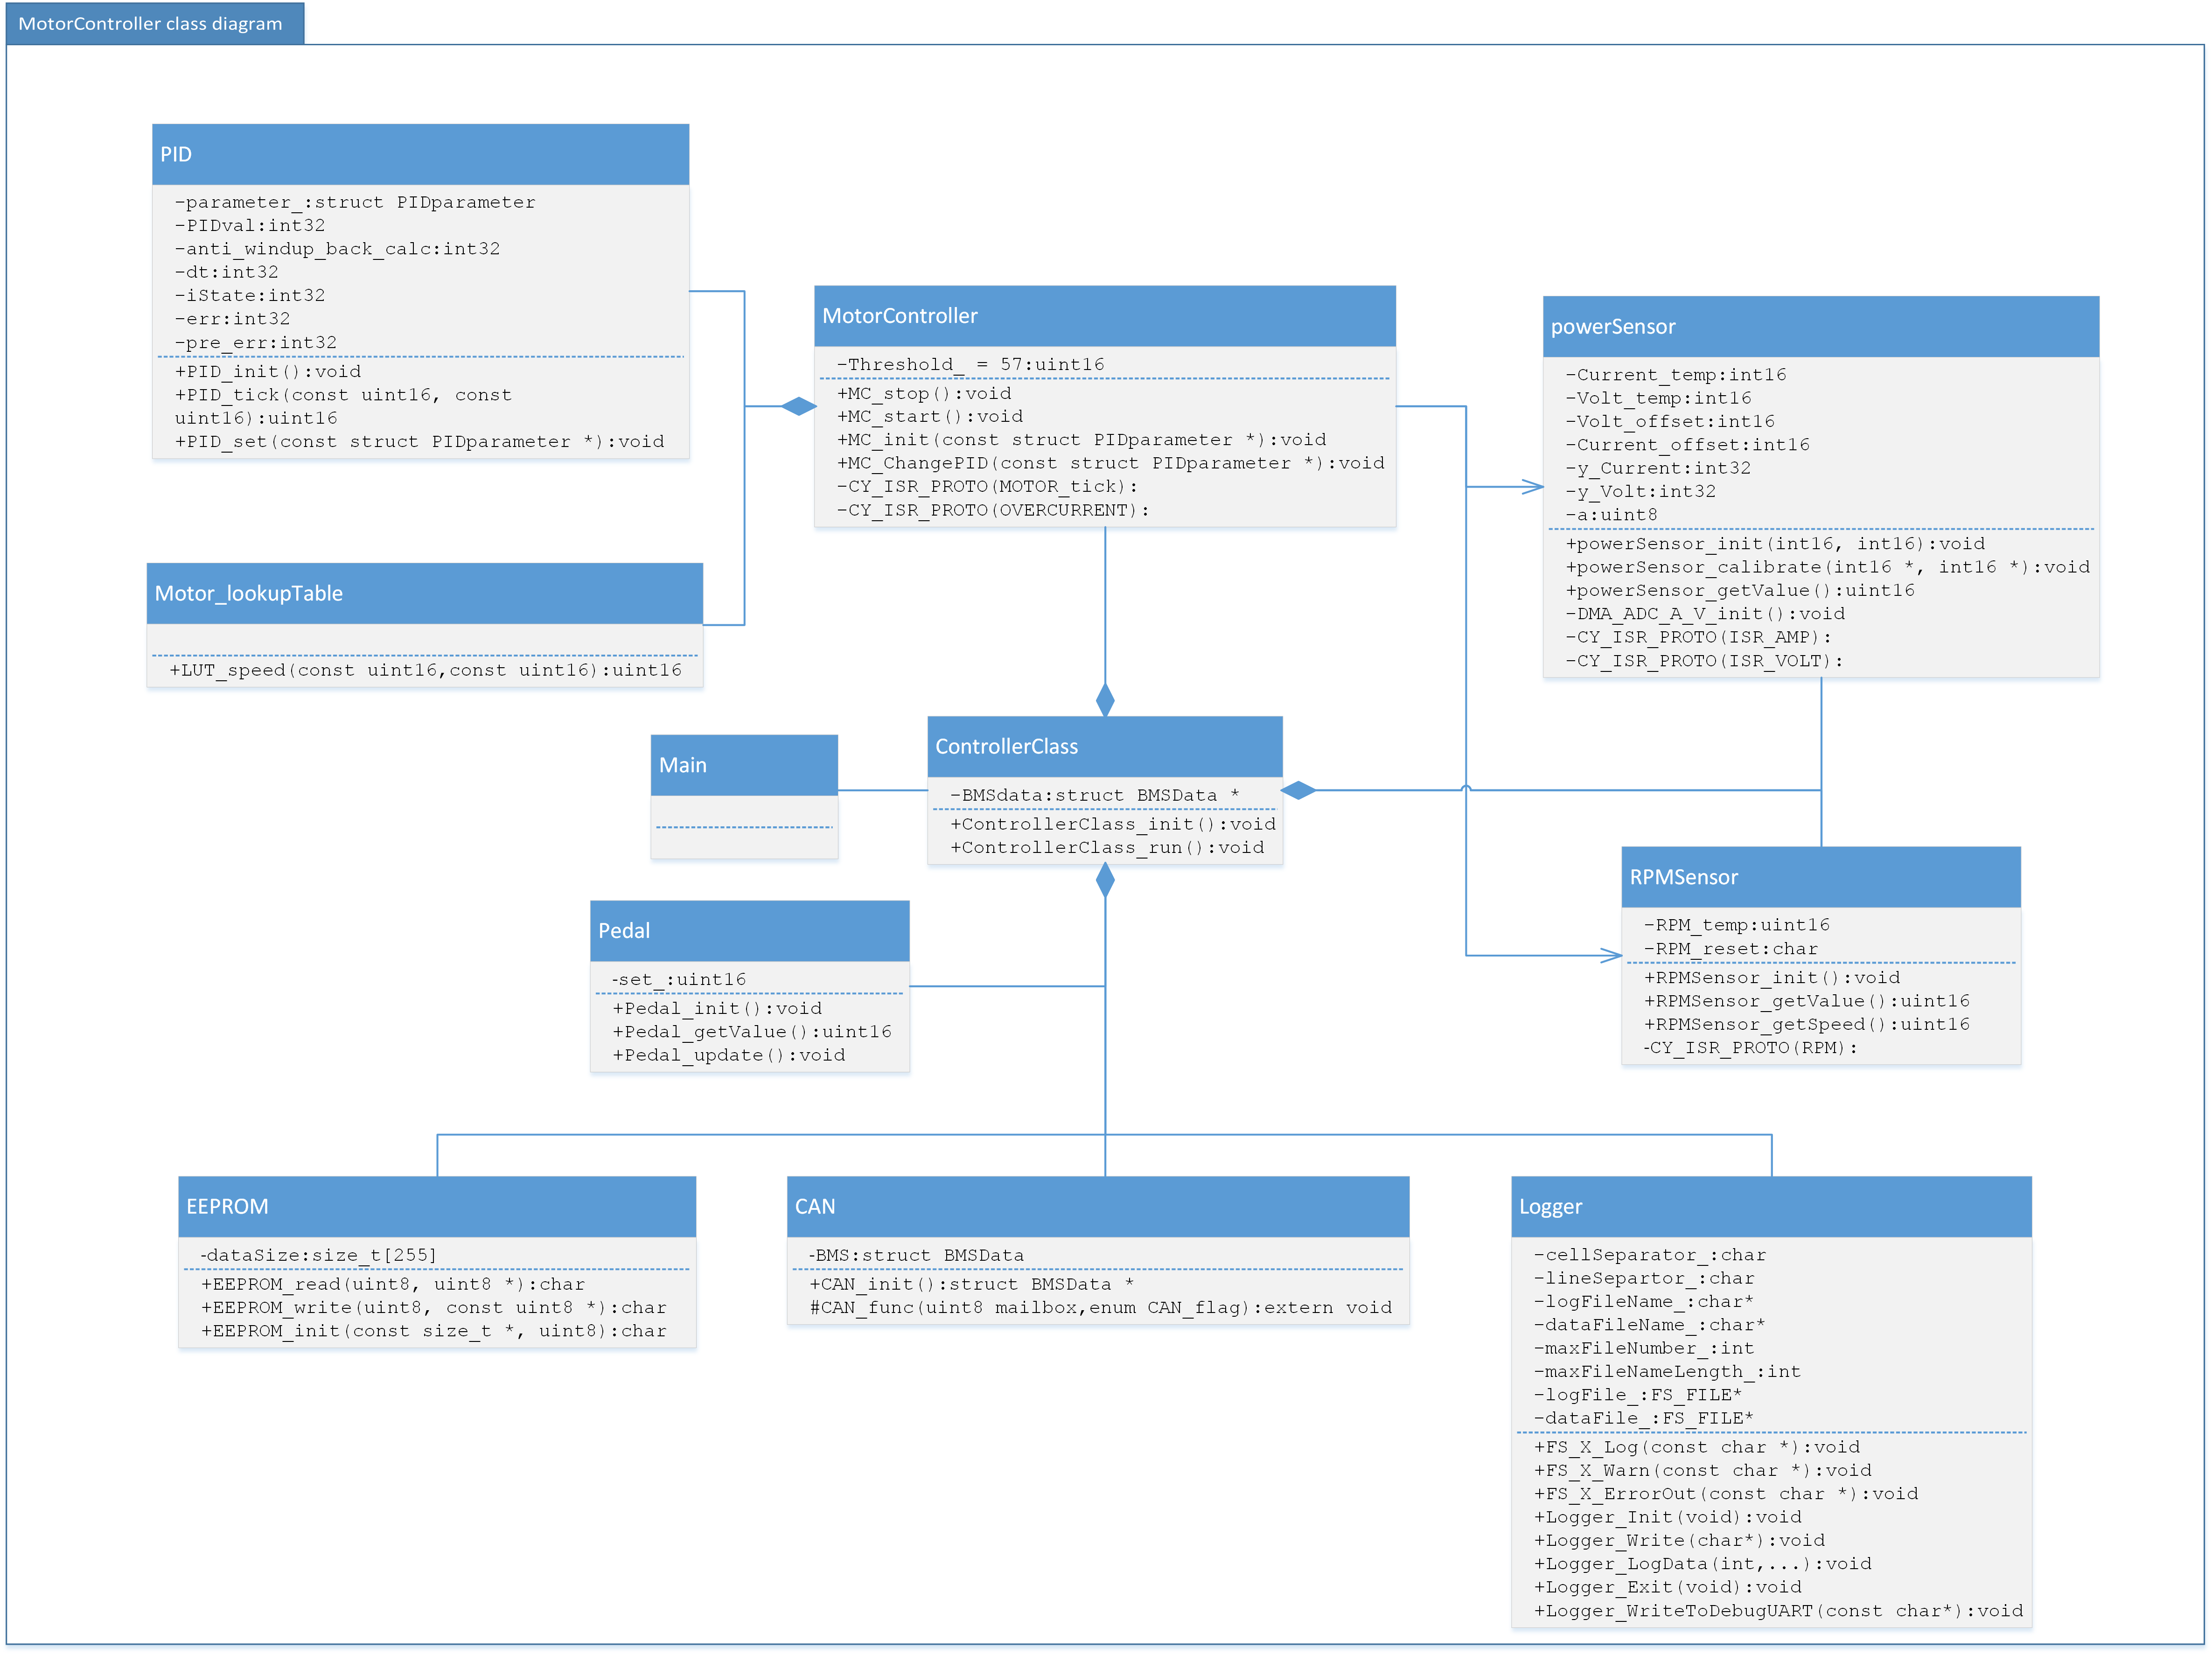
\includegraphics [width=6in]{Software/Pictures/class-diagram.png}
	\caption{Class diagram of the MCU}
	\label{fig:Class_diagram_MCU}
\end{figure}

The class diagram on figure \ref{fig:Class_diagram_MCU} gives a overlook over the classes in MCU. The controller class "ControllerClass" controls the main functionality and make sure what the sequencing are done right. The Controller-class job is to feed information to the motorController class and log data. It will collect all it data from both the local sensors and from the BMS through CAN.\\
MotorController class are controlling the motor and try to get the best efficiency as possible. To do what it has a Look up table "Motor\_lookUpTable" to find the best speed, for a specific Power. After, it will send the speed to PID regulator. The motorController has also build in a Coast and Burn see page \pageref{sec:Coast_and_Burn}\\

\subsection{Class description}

This sub section goes through all class in MCU, and give a overview over all methods.

\subsubsection{ControllerClass}

\begin{figure}[H]
	\centering
	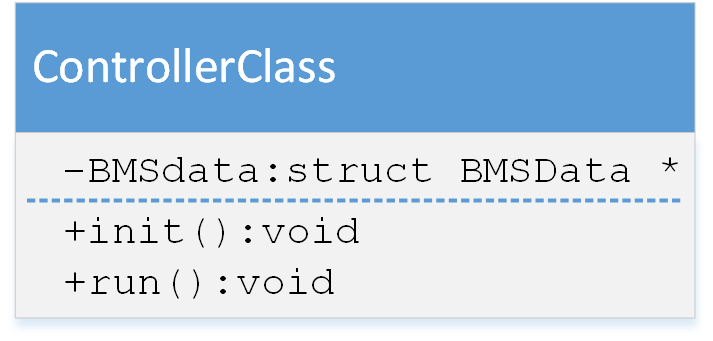
\includegraphics [width=2in]{Software/Pictures/class-diagram-controllerClass.png}
	\caption{ControllerClass class of MCU}
	\label{fig:Class_diagram_MCU_ControllerClass}
\end{figure}

\begin{table}[H]
	\centering
	\begin{tabular}{|p{5 cm}|p{10 cm}|}
		\hline
		\textbf{methods} & \textbf{Description} \\ \hline
		
		init
		& This method will initialize the entire MCU.
		\\ & \textbf{Parameter list ()}
		\\ & \textbf{Return parameter (void)}
		\\ \hline
		
		run
		& This method checking if there is some new status from the pedal, or have received new information from the BMS, if yes it will log the information. 
		\\ & \textbf{Parameter list ()}
		\\ & \textbf{Return parameter (void)}
		\\ \hline
		
	\end{tabular}
	\caption{Class description ControllerClass}
	\label{table:Class_description_ControllerClass_MCU}
\end{table}

\subsubsection{MotorController}

\begin{figure}[H]
	\centering
	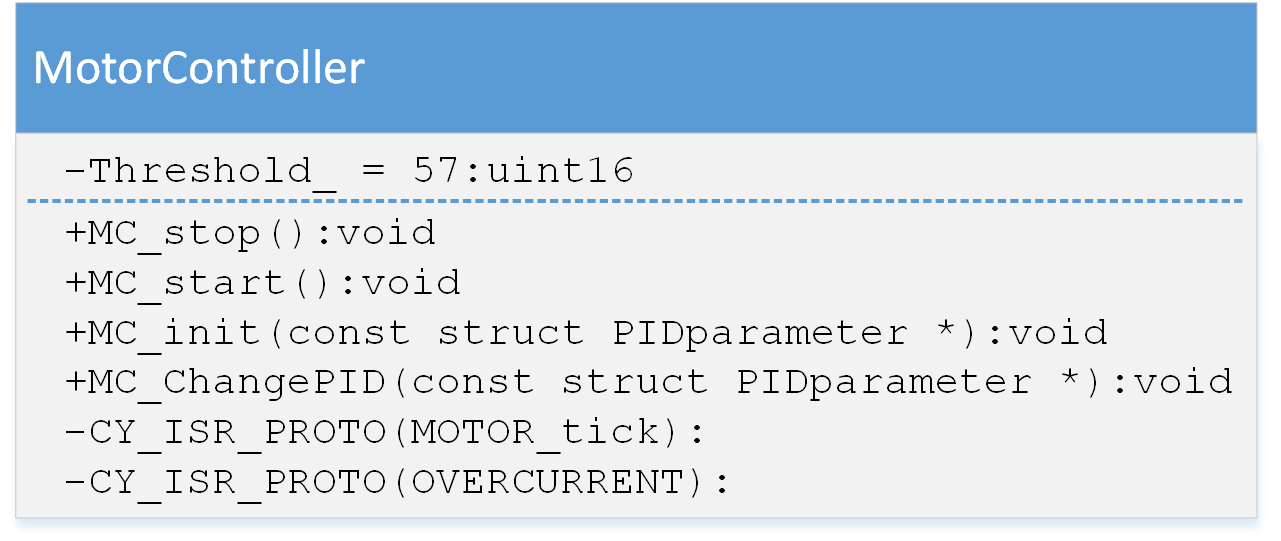
\includegraphics [width=3in]{Software/Pictures/class-diagram-motorControllerClass.png}
	\caption{motorController class of MCU}
	\label{fig:Class_diagram_MCU_motorControllerClass}
\end{figure}

\begin{table}[H]
	\centering
	\begin{tabular}{|p{5 cm}|p{10 cm}|}
		\hline
		\textbf{methods} & \textbf{Description} \\ \hline
		
		MC\_stop
		& Turn off the PWM signal to the motor.
		\\ & \textbf{Parameter list ()}
		\\ & \textbf{Return parameter (void)}
		\\ \hline
		
		MC\_start
		& Turn on the PWM signal to the motor.
		\\ & \textbf{Parameter list ()}
		\\ & \textbf{Return parameter ()}
		\\ \hline
		
		MC\_init
		& initializing the motorController class. 
		\\ & \textbf{Parameter list (const struct PIDparameter *)}
		\\ & \begin{itemize}
			\item {\large const struct PIDparameter *}
			\subitem \textit{A pointer to new PID parameters.}
		\end{itemize}
		\\ & \textbf{Return parameter (void)}
		\\ \hline
		
		MC\_changePID
		& Change the PID parameters in runtime.
		\\ & \textbf{Parameter list (const struct PIDparameter *)}
		\\ & \begin{itemize}
			\item {\large const struct PIDparameter *}
			\subitem \textit{The PID constants that will be used by the PID regulator.}
		\end{itemize}
		\\ & \textbf{Return parameter (void)}
		\\ \hline
		
		CY\_ISR(MOTOR\_tick)
		& It a interrupt routine that periodic update the PWM signal to the motor.
		\\ \hline
		
		CY\_ISR(OVERCURRENT)
		& If the "anti over current system" detects over-current, this routine will be launch. Note "anti over current system" is implemented on topdesign and will immediately turn off the PWM signal to the motor when it detect over-current.   
		\\ \hline
		
		
	\end{tabular}
	\caption{Class description motorController}
	\label{table:Class_description_motorController_MCU}
\end{table}

\subsubsection{EEPROM}

\begin{figure}[H]
	\centering
	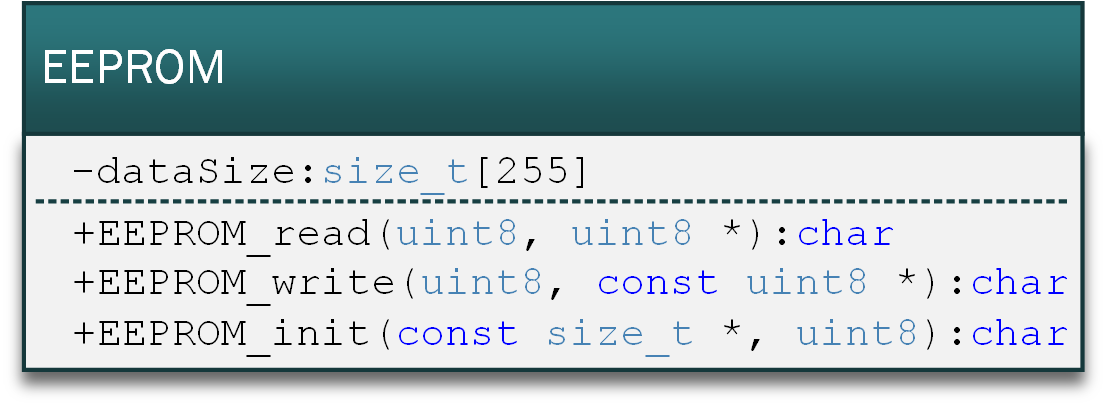
\includegraphics [width=3in]{../Documentation_RR/Software/Pictures/klassediagram_EEPROM.png}
	\caption{EEPROM class}
	\label{fig:Class_diagram_EEPROM}
\end{figure}


\begin{table}[H]
	\centering
	\begin{tabular}{|p{5 cm}|p{10 cm}|}
		\hline
		\textbf{methods} & \textbf{Description} \\ \hline
		
		EEPROM\_read
		& This method are used to read saved data from the EEPROM on the PSoC.
		\\ & \textbf{Return parameter}
		\\ & If the reading has succeeded it will return 1. If it fails to read from the EEPROM it return 0. Note it will also fail if there is no saved data.
		\\ & \textbf{Parameter list}
		\\ & \begin{itemize}
			\item {\large uint8}
			\subitem \textit{this parameter is used to choose the data you want to read, It just the ID of the content that has been saved.}
			\item {\large uint8*}
			\subitem \textit{A pointer to a buffer there the data will be saved to.}
		\end{itemize}
		\\ \hline
		
		EEPROM\_write
		& This method make it possible to save data to the EEPROM.
		\\ & \textbf{Return parameter}
		\\ & if it return 1, it has successfully write the data to the EEPROM. If it return -1 it has failed.
		\\ & \textbf{Parameter list}
		\\ & \begin{itemize}
			\item {\large uint8}
			\subitem \textit{this parameter is used to choose the data you want to save, It just the ID of the content you want to save.}
			\item {\large uint8*}
			\subitem \textit{A pointer to the data you want to saved. Note It will be a good idea to save it to the same data type, as you have defined in the initializing}
		\end{itemize}
		\\ \hline
		
		EEPROM\_init
		& It will initializing the class.
		\\ & \textbf{Return parameter}
		\\ & If it don't return 1, something is wrong and where is probably not enough memory in the EEPROM. If this method don't return 1 don't use the other methods!   
		\\ & \textbf{Parameter list}
		\\ & \begin{itemize}
			\item {\large const size\_t *}
			\subitem \textit{this parameter is used to send a array of sizes of data that will be saved on the EEPROM. The index of the arrays elements is also their IDs.}
			\item {\large uint8}
			\subitem \textit{This parameter is used to tell, have many elements there are in the array.}
		\end{itemize}
		\\ \hline
		
	\end{tabular}
	\caption{Class description EEPROM}
	\label{table:Class_description_EEPROM}
\end{table}

\subsubsection{Logger}

\begin{figure}[H]
	\centering
	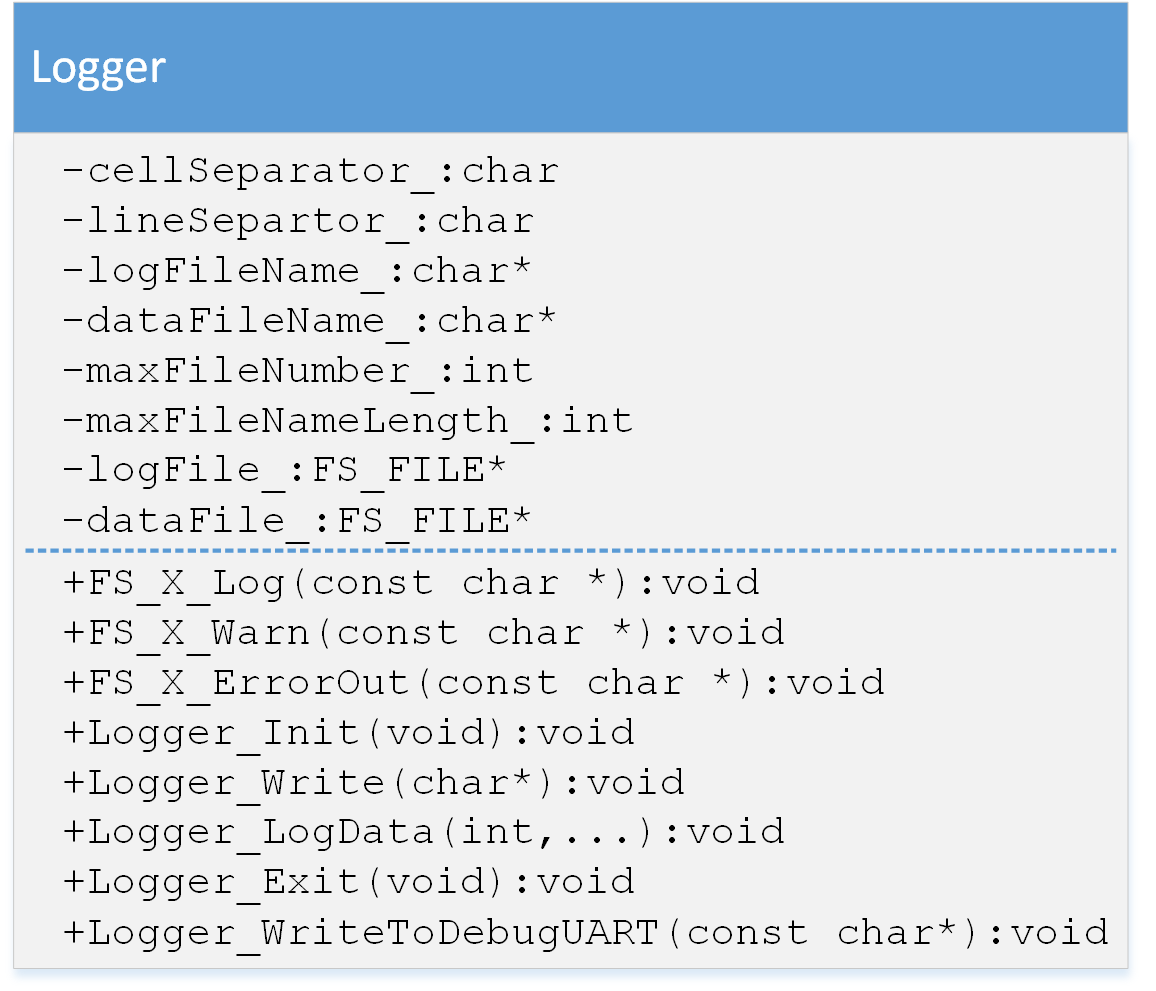
\includegraphics [width=3in]{Software/Pictures/class-diagram-logger.png}
	\caption{Logger class of MCU}
	\label{fig:Class_diagram_MCU_logger}
\end{figure}

\begin{table}[H]
	\centering
	\begin{tabular}{|p{5 cm}|p{10 cm}|}
		\hline
		\textbf{methods} & \textbf{Description} \\ \hline
		
		update
		& description
		\\ & \textbf{Parameter list (int8,int8)}
		\\ & \begin{itemize}
			\item {\large int8}
			\subitem \textit{something.}
		\end{itemize}
		\\ & \textbf{Return parameter (int8)}
		\\ & it will return .
		\\ \hline
		
	\end{tabular}
	\caption{Class description Logger}
	\label{table:Class_description_Logger_MCU}
\end{table}
\fxnote{Skal udfyldes}


\subsubsection{CAN}

\begin{figure}[H]
	\centering
	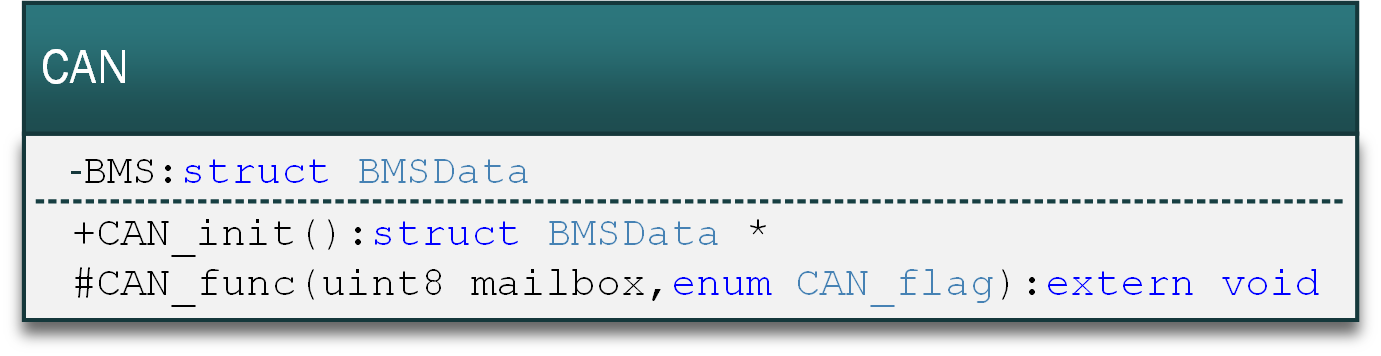
\includegraphics [width=4in]{Software/Pictures/class-diagram-CAN.png}
	\caption{CAN class of MCU}
	\label{fig:Class_diagram_MCU_CAN}
\end{figure}

\begin{table}[H]
	\centering
	\begin{tabular}{|p{5 cm}|p{10 cm}|}
		\hline
		\textbf{methods} & \textbf{Description} \\ \hline
		
		CAN\_init
		& Initializing CAN. 
		\\ & \textbf{Parameter list ()}
		\\ & \textbf{Return parameter (void)}
		\\ \hline
		
		CAN\_func
		& Control all received messages.
		\\ & \textbf{Parameter list (uint8, enum CAN\_flag)}
		\\ & \begin{itemize}
			\item {\large uint8}
			\subitem \textit{the mailbox number.}
			\item {\large enum CAN\_flag}
			\subitem \textit{A flag that tells what kind of message has been received.}
		\end{itemize}
		\\ & \textbf{Return parameter (void)}
		\\ \hline
		
		
	\end{tabular}
	\caption{Class description ControllerClass}
	\label{table:Class_description_CAN_MCU}
\end{table}

\subsubsection{RPMSensor}

\begin{figure}[H]
	\centering
	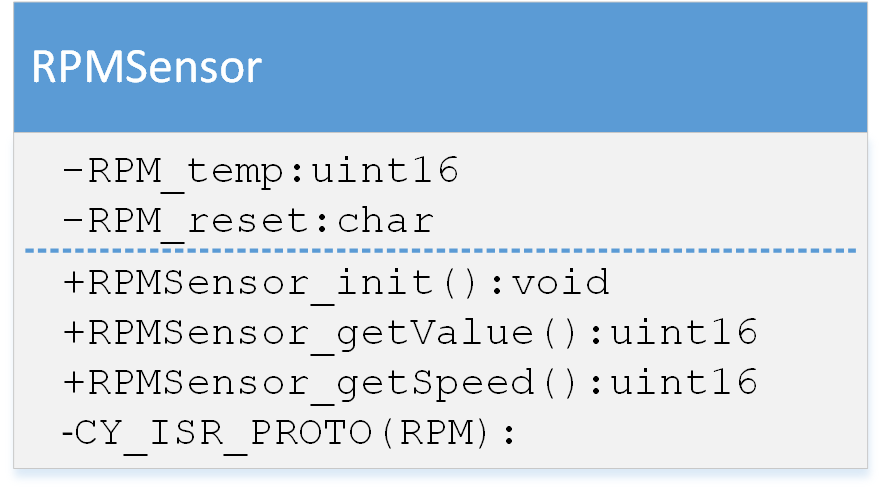
\includegraphics [width=2in]{Software/Pictures/class-diagram-RPMSensor.png}
	\caption{RPMSensor class of MCU}
	\label{fig:Class_diagram_MCU_RPMSensor}
\end{figure}

\begin{table}[H]
	\centering
	\begin{tabular}{|p{5 cm}|p{10 cm}|}
		\hline
		\textbf{methods} & \textbf{Description} \\ \hline
		
		RPMSensor\_init
		& Initializing the sensor. 
		\\ & \textbf{Parameter list ()}
		\\ & \textbf{Return parameter (void)}
		\\ \hline
		
		RPMSensor\_getValue
		& Gets the RPM value.
		\\ & \textbf{Parameter list ()}
		\\ & \textbf{Return parameter (uint16)}
		\\ & return the RPM value. LSB = 0.1 RPM.
		\\ \hline

		RPMSensor\_getSpeed
		& Gets the speed in $ \frac{m}{s} $.
		\\ & \textbf{Parameter list ()}
		\\ & \textbf{Return parameter (uint16)}
		\\ & return the Speed. Not finish. Will just return RPM value.
		\\ \hline
		
		CY\_ISR(RPM)
		& The interrupt routine that measure the speed.
		\\ \hline
		
	\end{tabular}
	\caption{Class description RPMSensor}
	\label{table:Class_description_RPMSensor_MCU}
\end{table}

\subsubsection{powerSensor}

\begin{figure}[H]
	\centering
	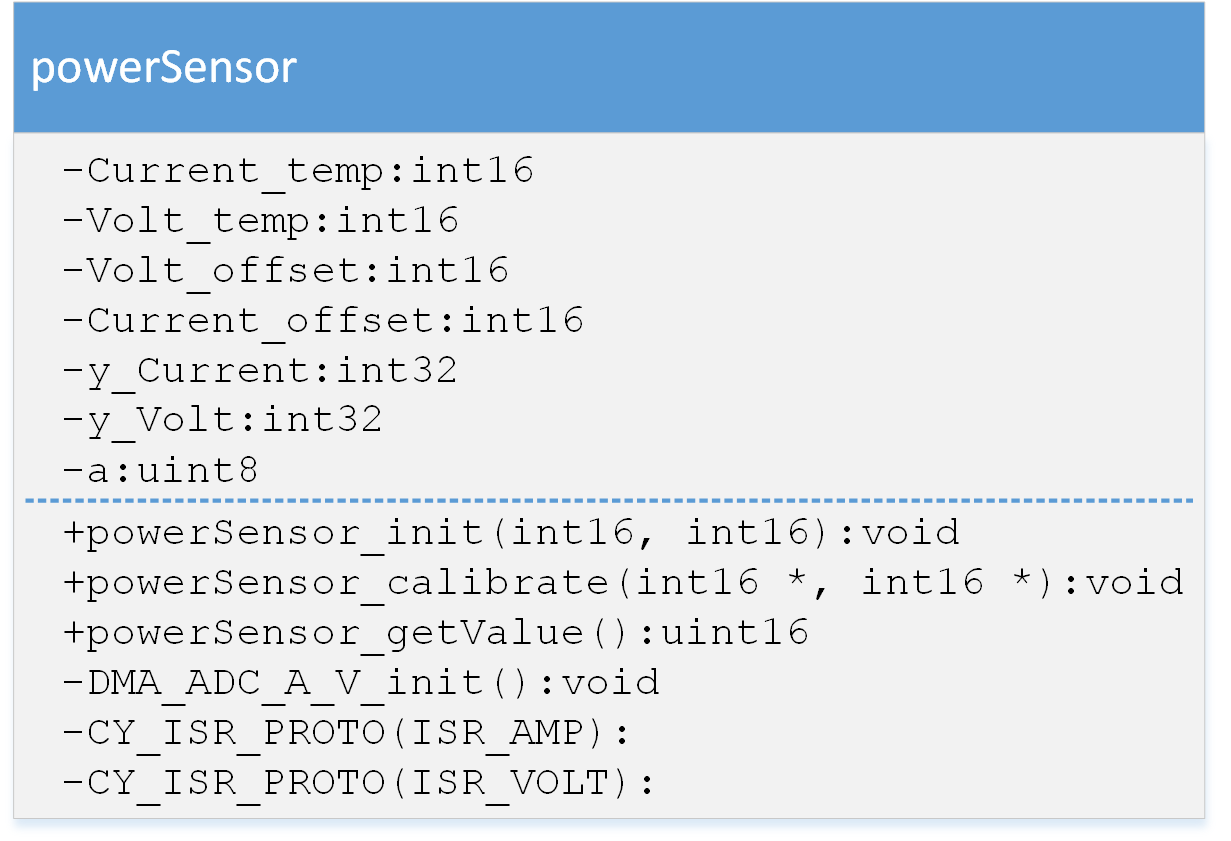
\includegraphics [width=3in]{Software/Pictures/class-diagram-powerSensor.png}
	\caption{powerSensor class of MCU}
	\label{fig:Class_diagram_MCU_powerSensor}
\end{figure}

\begin{table}[H]
	\centering
	\begin{tabular}{|p{5 cm}|p{10 cm}|}
		\hline
		\textbf{methods} & \textbf{Description} \\ \hline
		
		powerSensor\_init
		& Initializing the sensor
		\\ & \textbf{Parameter list (int16,int16)}
		\\ & \begin{itemize}
			\item {\large int16}
			\subitem \textit{Offset value for the voltage sensor.}
			\item {\large int16}
			\subitem \textit{Offset value for the current sensor.}
		\end{itemize}
		\\ & \textbf{Return parameter (void)}
		\\ \hline
		
		powerSensor\_calibrate
		& Calibrate the sensor, and return offset values through the parameter list.
		\\ & \textbf{Parameter list (int16 *,int16 *)}
		\\ & \begin{itemize}
			\item {\large int16 *}
			\subitem \textit{return voltage offset value.}
			\item {\large int16 *}
			\subitem \textit{return current offset value}
		\end{itemize}
		\\ & \textbf{Return parameter (void)}
		\\ \hline
		
		powerSensor\_getValue
		& Return the power usage.
		\\ & \textbf{Parameter list ()}
		\\ & \textbf{Return parameter (uint16)}
		\\ & Return the power usage. $ LSB = \SI{0.1}{\watt} $
		\\ \hline
		
		DMA\_ADC\_A\_V\_init
		& DMA setup of the sensors.
		\\ & \textbf{Parameter list ()}
		\\ & \textbf{Return parameter (void)}
		\\ \hline
		
		CY\_ISR(ISR\_AMP)
		& The interrupt routine that capture the current.
		\\ \hline
		
		CY\_ISR(ISR\_VOLT)
		& The interrupt routine that capture the voltage.
		\\ \hline
		
	\end{tabular}
	\caption{Class description powerSensor}
	\label{table:Class_description_MCU_powerSensor}
\end{table}


\subsubsection{Pedal}

\begin{figure}[H]
	\centering
	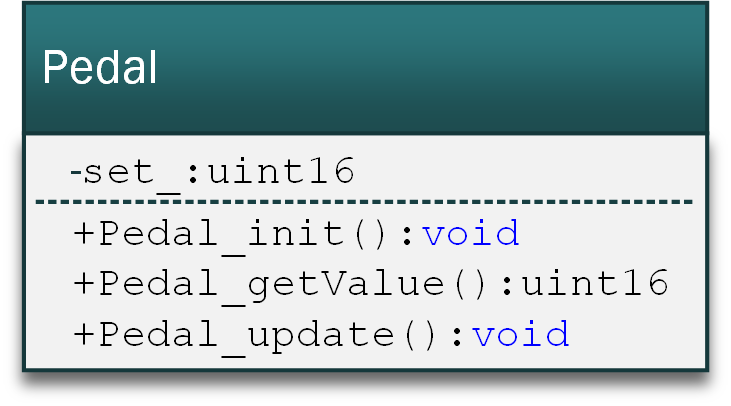
\includegraphics [width=2in]{Software/Pictures/class-diagram-pedal.png}
	\caption{pedal class of MCU}
	\label{fig:Class_diagram_MCU_pedal}
\end{figure}

\begin{table}[H]
	\centering
	\begin{tabular}{|p{5 cm}|p{10 cm}|}
		\hline
		\textbf{methods} & \textbf{Description} \\ \hline
		
		Pedal\_init
		& Initializing the pedal.
		\\ & \textbf{Parameter list ()}
		\\ & \textbf{Return parameter (void)}
		\\ \hline
		
		Pedal\_getValue
		& Gets the value of the pedal.
		\\ & \textbf{Parameter list ()}
		\\ & \textbf{Return parameter (uint16)}
		\\ & return the wanted speed. $ LSB = \SI{0.1}{rpm} $
		\\ \hline
		
		Pedal\_update
		& refresh the value of the pedal. 
		\\ & \textbf{Parameter list ()}
		\\ & \textbf{Return parameter (void)}
		\\ \hline
		
	\end{tabular}
	\caption{Class description pedal}
	\label{table:Class_description_MCU_pedal}
\end{table}

\subsubsection{PID}

\begin{figure}[H]
	\centering
	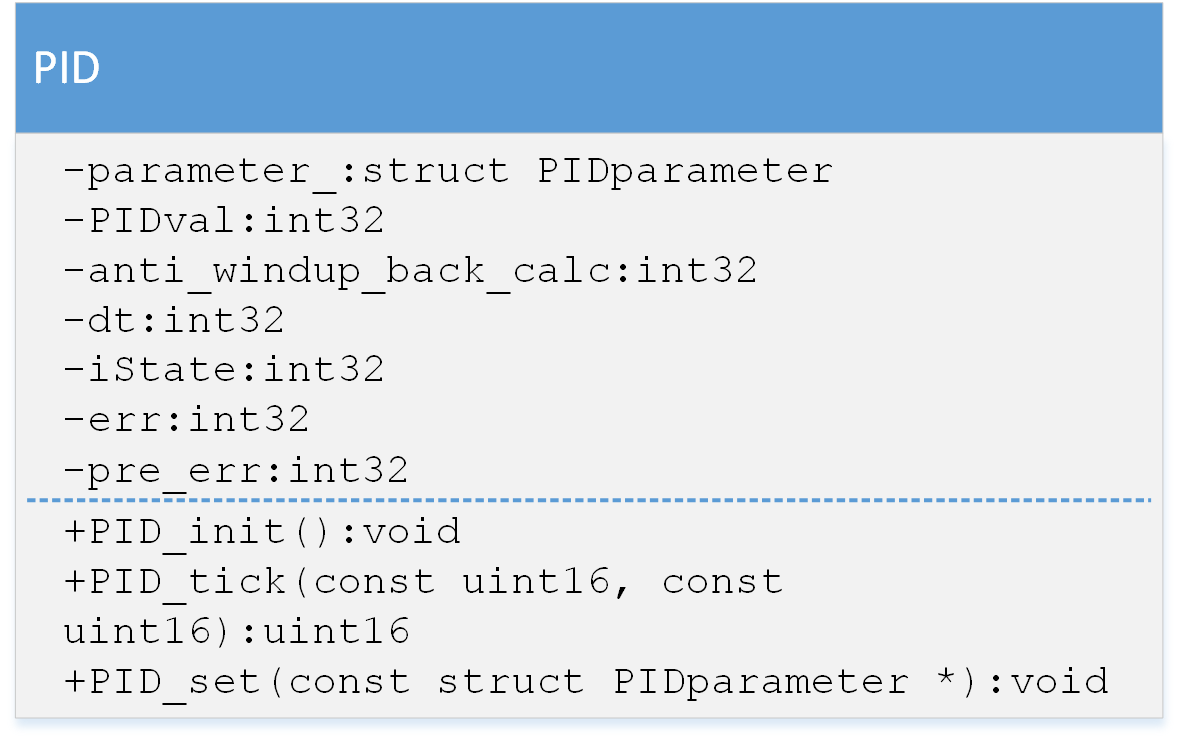
\includegraphics [width=3in]{Software/Pictures/class-diagram-PID.png}
	\caption{PID class of MCU}
	\label{fig:Class_diagram_MCU_PID}
\end{figure}

\begin{table}[H]
	\centering
	\begin{tabular}{|p{5 cm}|p{10 cm}|}
		\hline
		\textbf{methods} & \textbf{Description} \\ \hline
		
		PID\_init
		& Initializing PID regulator.
		\\ & \textbf{Parameter list ()}
		\\ & \textbf{Return parameter (void)}
		\\ \hline
		
		PID
		& Where the PID calculation happens.
		\\ & \textbf{Parameter list (const uint16, const uint16)}
		\\ & \begin{itemize}
			\item {\large uint16}
			\subitem \textit{wanted speed}
			\item {\large uint16}
			\subitem \textit{Measured speed}
		\end{itemize}
		\\ & \textbf{Return parameter (uint16)}
		\\ & Return the bit value for the PWM signal to the motor.
		\\ \hline
		
		setPID
		& Set the PID parameter.
		\\ & \textbf{Parameter list (const struct PIDparameter *)}
		\\ & \begin{itemize}
			\item {\large const struct PIDparameter *}
			\subitem \textit{The PID parameter}
		\end{itemize}
		\\ & \textbf{Return parameter (void)}
		\\ \hline
		
	\end{tabular}
	\caption{Class description ControllerClass}
	\label{table:Class_description_MCU_PID}
\end{table}

\subsubsection{LUT - look up table}

\begin{figure}[H]
	\centering
	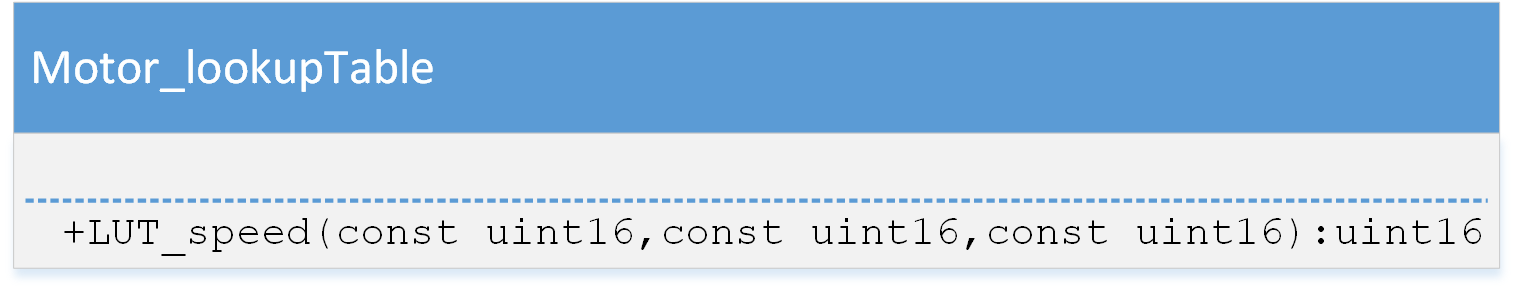
\includegraphics [width=3in]{Software/Pictures/class-diagram-LUT.png}
	\caption{Motor\_lookupTable class of MCU}
	\label{fig:Class_diagram_MCU_LUT}
\end{figure}

\begin{table}[H]
	\centering
	\begin{tabular}{|p{5 cm}|p{10 cm}|}
		\hline
		\textbf{methods} & \textbf{Description} \\ \hline
		
		LUT\_speed
		& A 2D look up table what will return the best speed from the power usage.
		\\ & \textbf{Parameter list (const uint16, const uint16, const uint16)}
		\\ & \begin{itemize}
			\item {\large const uint16}
			\subitem \textit{The wanted speed.}
			\item {\large const uint16}
			\subitem \textit{The currently speed.}
			\item {\large const uint16}
			\subitem \textit{The currently power usage.}
		\end{itemize}
		\\ & \textbf{Return parameter (uint16)}
		\\ & return the best speed to get the best efficiency.
		\\ \hline
		
	\end{tabular}
	\caption{Class description look up table}
	\label{table:Class_description_MCU_LUT}
\end{table}

%\label{sec:Coast_and_Burn} \fxnote{fix pageref}
